\chapter{Introducción}
\hrule \bigskip \vspace*{1cm}
%------------------------------------------------------------------------

\label{sec:introduccion}

Este capítulo presenta el problema abordado por la tesis y la propuesta desarrollada para resolverlo. La Sección~\ref{sec:contexto} sitúa el problema en el contexto de la gestión de riesgos financieros, y la Sección~\ref{sec:motivacion} expone por qué la falta de explicabilidad de los modelos de aprendizaje automático es un problema práctico y regulatorio. La Sección~\ref{sec:planteamiento_problema} formaliza la brecha específica que ningún método previo cubre. La Sección~\ref{sec:justificacion} justifica la propuesta frente a las limitaciones de los trabajos más cercanos. Las Secciones~\ref{sec:objetivo_general} y \ref{sec:objetivos_especificos} presentan el objetivo general, con el flujo del framework, y los objetivos específicos que guían el trabajo. Finalmente, la Sección~\ref{sec:organizacion_tesis} describe la organización del resto del documento.

\section{Contexto}
\label{sec:contexto}

La predicción de series temporales financieras, como el precio de cierre diario de un índice bursátil, se usa en la práctica para decidir directamente sobre un portafolio, cuándo comprar, mantener o vender una posición, o cuánto capital asignar a un activo frente a otro \cite{arsenault2025}. El riesgo financiero relevante para esta tesis es exactamente esa traducción, la pérdida de valor que se materializa sobre el portafolio cuando la decisión se apoyó en una predicción que resultó incorrecta. Estas consecuencias no son solo teóricas. Cohen et al.\ \cite{cohen2023blackbox} documentan que la opacidad de los modelos de aprendizaje automático usados para generar esas predicciones agrega una segunda capa a ese riesgo, el \emph{riesgo de modelo} (\emph{model risk}), definido por el propio SR~11-7 \cite{sr117} como el riesgo de consecuencias adversas derivadas de decisiones basadas en resultados de modelos incorrectos o mal utilizados. A diferencia del riesgo de que el precio se mueva en contra, que existe incluso con un modelo perfectamente entendido, el riesgo de modelo existe porque nadie puede validar si el modelo aprendió una relación económica real o una coincidencia sin significado presente en los datos de entrenamiento, hasta que la decisión ya se tomó. Esta tesis se ubica específicamente en el riesgo de modelo, no en el riesgo de que el mercado se mueva en contra. Este riesgo no es hipotético dentro del propio trabajo, la consistencia entre modelos que se mide como criterio de validación (Sección~\ref{sec:estrategia_validacion}) resulta sistemáticamente menor durante el régimen bajista de 2022 que durante el régimen alcista de 2023 y 2024 (Capítulo~5), es decir, el desacuerdo entre modelos sobre qué variables importan aumenta justo en el escenario donde una decisión errónea es más costosa para una institución.

\section{Motivación}
\label{sec:motivacion}

En los últimos años, los modelos de aprendizaje profundo han reducido el error de predicción sobre este tipo de datos frente a métodos estadísticos clásicos \cite{bhandari2022, abdulquadir2023}. Sin embargo, estos modelos no explican por qué llegan a cada resultado, y esa falta de explicación ya tiene consecuencias regulatorias concretas. El SR 11-7 de la Reserva Federal estadounidense \cite{sr117} obliga a los bancos a demostrar que entienden las capacidades y los límites de cada modelo antes de usarlo. El Reglamento de Inteligencia Artificial de la Unión Europea \cite{euaiact2024} exige, para ciertos usos financieros como la evaluación crediticia, que el modelo sea lo bastante transparente para que quien lo usa pueda interpretar sus resultados. Pese a estas exigencias, Sovrano et al.\ \cite{sovrano2026} muestran que los métodos de explicabilidad actuales todavía no las cumplen de forma sistemática.

Para abordar esta opacidad, el campo de la Inteligencia Artificial Explicable (XAI) agrupa métodos que permiten identificar qué factores influyeron en una predicción. Estos métodos se organizan en familias según su mecanismo. Los basados en gradientes, como DeepLIFT \cite{shrikumar2017}, requieren acceso a la estructura interna del modelo. Los basados en atención dependen de la arquitectura utilizada, y su equivalencia con una explicación es discutida \cite{jain2019}. Los basados en perturbación, como SHAP y LIME, son agnósticos al modelo porque generan explicaciones observando cómo cambia la salida al modificar partes de la entrada \cite{arsenault2025}. Esta capacidad no depende de ninguna propiedad especial del modelo, solo requiere poder consultarlo como una función que recibe una entrada y devuelve una predicción, sin inspeccionar pesos ni gradientes, por lo que el mismo mecanismo se aplica sin modificación tanto a una red neuronal como a un modelo de ensamble o a un modelo estadístico clásico. El costo de esa generalidad es que, a diferencia de un método de gradiente que obtiene la sensibilidad local en una sola operación analítica, un método de perturbación necesita consultar el modelo una vez por cada elemento de la entrada cuya influencia quiere medir. No obstante, estos últimos asumen, en su formulación habitual, que las variables de entrada son independientes entre sí \cite{lundberg2017, ribeiro2016}. Al aplicarse sobre series temporales, tratan cada paso de tiempo como una variable aislada, ignorando que las observaciones forman una secuencia con dependencias estructurales \cite{tonekaboni2020, huang2025}.

Construir un framework de explicabilidad para este dominio conlleva responsabilidades éticas concretas, no solo declarativas. Un modelo entrenado sobre datos financieros históricos hereda los sesgos de ese historial, un régimen de mercado específico \cite{angtimmermann2012}, la composición cambiante del índice, la autocorrelación trivial del precio \cite{fama1970, meese1983}, y una explicación poco fiel puede ocultar esos sesgos en vez de exponerlos \cite{rudin2019}. Por esta razón, este trabajo reporta también los resultados que no favorecen a la propuesta, que ningún modelo entrenado supera el baseline de persistencia ingenua y que la consideración específica investigada para Random Forest (Sección~\ref{sec:leaf_reference_propuesta}) no confirmó la hipótesis inicial, en vez de omitirlos. Además, al no requerir gradientes ni una optimización costosa por instancia, el framework reduce la barrera computacional y de infraestructura para auditar modelos financieros, una consideración de acceso equitativo relevante para instituciones o reguladores sin la capacidad de cómputo que exigen métodos como Shapley Value Sampling o las máscaras aprendidas por gradiente, y reduce a la vez el costo energético asociado a esa auditoría.

\section{Planteamiento del Problema}
\label{sec:planteamiento_problema}

El problema que aborda esta tesis puede formularse como un problema de cómputo con dos requisitos que ningún método previo satisface a la vez. Primero, que el mecanismo de explicación funcione sobre arquitecturas de naturaleza computacional distinta sin acceder a su implementación interna. Segundo, que ese mecanismo tenga un costo fijo por instancia, evaluable en una sola pasada, sin resolver una optimización propia cada vez que se explica una predicción.

Los métodos con acceso a la estructura interna del modelo logran coherencia temporal en la atribución pero quedan acoplados a una arquitectura específica, los pesos de atención de un Transformer no tienen equivalente en un modelo de ensamble como Random Forest \cite{arsenault2025}. Los métodos de perturbación agnósticos sí funcionan sobre cualquier modelo, pero generan perturbaciones que rompen la dependencia estructural entre observaciones consecutivas \cite{tonekaboni2020, huang2025}.

Existen métodos que respetan el orden temporal, como las máscaras dinámicas de Crabbé y Van Der Schaar \cite{crabbe2021}, pero ajustan la perturbación resolviendo, para cada instancia, un problema de optimización no convexo mediante descenso de gradiente, lo que además de un costo computacional considerable les impide operar sobre modelos no diferenciables como Random Forest. Dos extensiones directas de este método, publicadas en ICML \cite{enguehard2023} e ICLR \cite{liu2024contralsp}, corrigen la calidad de la perturbación pero mantienen la misma dependencia del gradiente. Cinco años después de la propuesta original, ningún método de esta línea de trabajo funciona sin gradientes, y ninguno se ha validado sobre series financieras pese a mencionarlas como motivación. Random Forest es, en este sentido, el caso concreto que hace tangible el problema, sigue siendo estado del arte en datos tabulares \cite{grinsztajn2022}, y es precisamente el tipo de modelo que esta línea de trabajo excluye por diseño.

El costo fijo por instancia que exige el segundo requisito no es una meta de eficiencia aislada, depende directamente de cómo se resuelva el primer requisito. Las máscaras dinámicas de Crabbé y Van Der Schaar \cite{crabbe2021} son intrínsecamente secuenciales, cada paso del descenso de gradiente parte del resultado del paso anterior, así que su costo por instancia crece con el número de iteraciones que necesite converger y no puede reducirse agrupando esas iteraciones en una sola operación. El mecanismo de perturbación agnóstico que exige el primer requisito tiene, en cambio, una propiedad distinta, perturbar la celda $(t,v)$ para medir su influencia no depende del resultado de perturbar ninguna otra celda $(t',v')$. Al no existir esa dependencia entre perturbaciones, todas pueden evaluarse en un único conjunto de consultas al modelo procesado de una vez, en vez de una secuencia de pasos donde cada uno espera al anterior. Por esta razón el framework propuesto en esta tesis no necesita diseñarse ni optimizarse aparte para ejecutar en paralelo, la independencia entre perturbaciones que exige la agnosticidad hace que la versión de una sola pasada sea, al mismo tiempo, la versión paralela.

\subsection{Estrategia de validación}
\label{sec:estrategia_validacion}

La independencia entre perturbaciones descrita en el párrafo anterior también define cómo se valida la propuesta a lo largo de la tesis, en dos etapas con una naturaleza distinta cada una.

La primera etapa usa datos sintéticos generados por una función matemática definida por la propia investigadora, no aprendida ni etiquetada externamente. La función se construye de forma que su salida dependa matemáticamente solo de un subconjunto pequeño y conocido de celdas $(t,v)$ de la ventana de entrada, por ejemplo $f(X) = \sum_{(t,v) \in A} x_{t,v}^2$, donde $A$ es ese subconjunto elegido de antemano. El resto de las celdas de $X$ no aparece en la fórmula, así que no puede influir en la salida. Como la función es propia, el conjunto $A$ de celdas relevantes se conoce con certeza, y sirve como ground truth contra el cual comparar la matriz de importancia que produce el framework, esa comparación es la que permite calcular métricas de precisión y cobertura como AUP y AUR (Capítulo~5). Esta es la misma estrategia que usó DynaMask con sus propios datasets sintéticos \cite{crabbe2021}, la diferencia con esta tesis está en el dominio de la función construida, no en el mecanismo de validación.

La segunda etapa usa el S\&P~500 real, donde no existe una función conocida que genere el precio del día siguiente y, por lo tanto, tampoco existe un conjunto $A$ verdadero contra el cual comparar. Al no haber ground truth, la validación deja de medir precisión directa y pasa a depender de señales indirectas de que la explicación refleja el comportamiento real del modelo y no un artefacto del método \cite{adebayo2018}, que las atribuciones sean estadísticamente distintas de una asignación aleatoria, que sean consistentes entre modelos de mecanismo similar y menos consistentes entre modelos de mecanismo distinto (objetivo específico 4), y que se mantengan estables frente a variaciones del propio procedimiento, el orden temporal de la perturbación, el vector de referencia usado y el régimen de mercado evaluado. Esta segunda etapa es la que corresponde específicamente al dominio y al tema de estudio de esta tesis, series temporales financieras sin ground truth disponible, y es donde el aporte de validación es más propio del trabajo.

\section{Justificación}
\label{sec:justificacion}

Los trabajos relacionados descritos en los párrafos anteriores resuelven, cada uno, solo uno de los dos requisitos planteados en el Planteamiento del Problema (Sección~\ref{sec:planteamiento_problema}), nunca ambos a la vez. Los métodos de perturbación agnósticos como SHAP y LIME satisfacen el primer requisito, funcionan sobre cualquier arquitectura sin acceder a su interior, pero no el segundo, porque al tratar cada paso de tiempo como una variable independiente rompen el orden temporal de la serie \cite{tonekaboni2020, huang2025}. Las máscaras dinámicas de Crabbé y Van Der Schaar \cite{crabbe2021} y sus extensiones en ICML \cite{enguehard2023} e ICLR \cite{liu2024contralsp} satisfacen el segundo requisito en cuanto a coherencia temporal, pero no el primero, porque su optimización por descenso de gradiente las ata a modelos diferenciables y excluye por diseño a modelos no diferenciables como Random Forest. Ninguno de los dos grupos ha sido validado además sobre series financieras pese a mencionarlas como motivación.

El motor de perturbaciones temporales propuesto en esta tesis (Capítulo~4) se diseña precisamente para cerrar esa brecha compartiendo la propiedad que las máscaras dinámicas no tienen y que los métodos agnósticos clásicos tampoco tienen en su formulación original. Perturba una sola celda $(t,v)$ a la vez, dejando el resto de la ventana exactamente en su valor y posición observados, lo que preserva el orden temporal sin necesidad de gradientes ni de una optimización propia por instancia. Esta decisión de diseño es la que permite explicar bajo el mismo mecanismo a los tres modelos entrenados en esta tesis, LSTM, Transformer y Random Forest, y es la que se somete a verificación empírica en el Capítulo~5, tanto contra un ground truth sintético conocido como sobre el S\&P~500 real.

\section{Objetivo General}
\label{sec:objetivo_general}

Desarrollar un framework de explicabilidad temporal agnóstico al modelo para la predicción de series temporales financieras, que atribuya importancia por variable y paso de tiempo sin depender de la estructura interna del modelo explicado ni requerir acceso a sus gradientes, y cuyo costo de cómputo por instancia sea fijo y evaluable en una sola pasada paralela, sin resolver una optimización propia para cada predicción explicada.

El flujo completo del framework se resume en la Figura~\ref{fig:pipeline} y se detalla en el Capítulo~4. Los datos de entrada y su preparación, en azul, alimentan a un modelo predictivo, en verde, que se conecta con el motor de perturbación mediante una interfaz uniforme de predicción. El motor, en naranja, es la contribución principal y produce la matriz de importancia temporal.

\begin{figure}[ht]
\centering
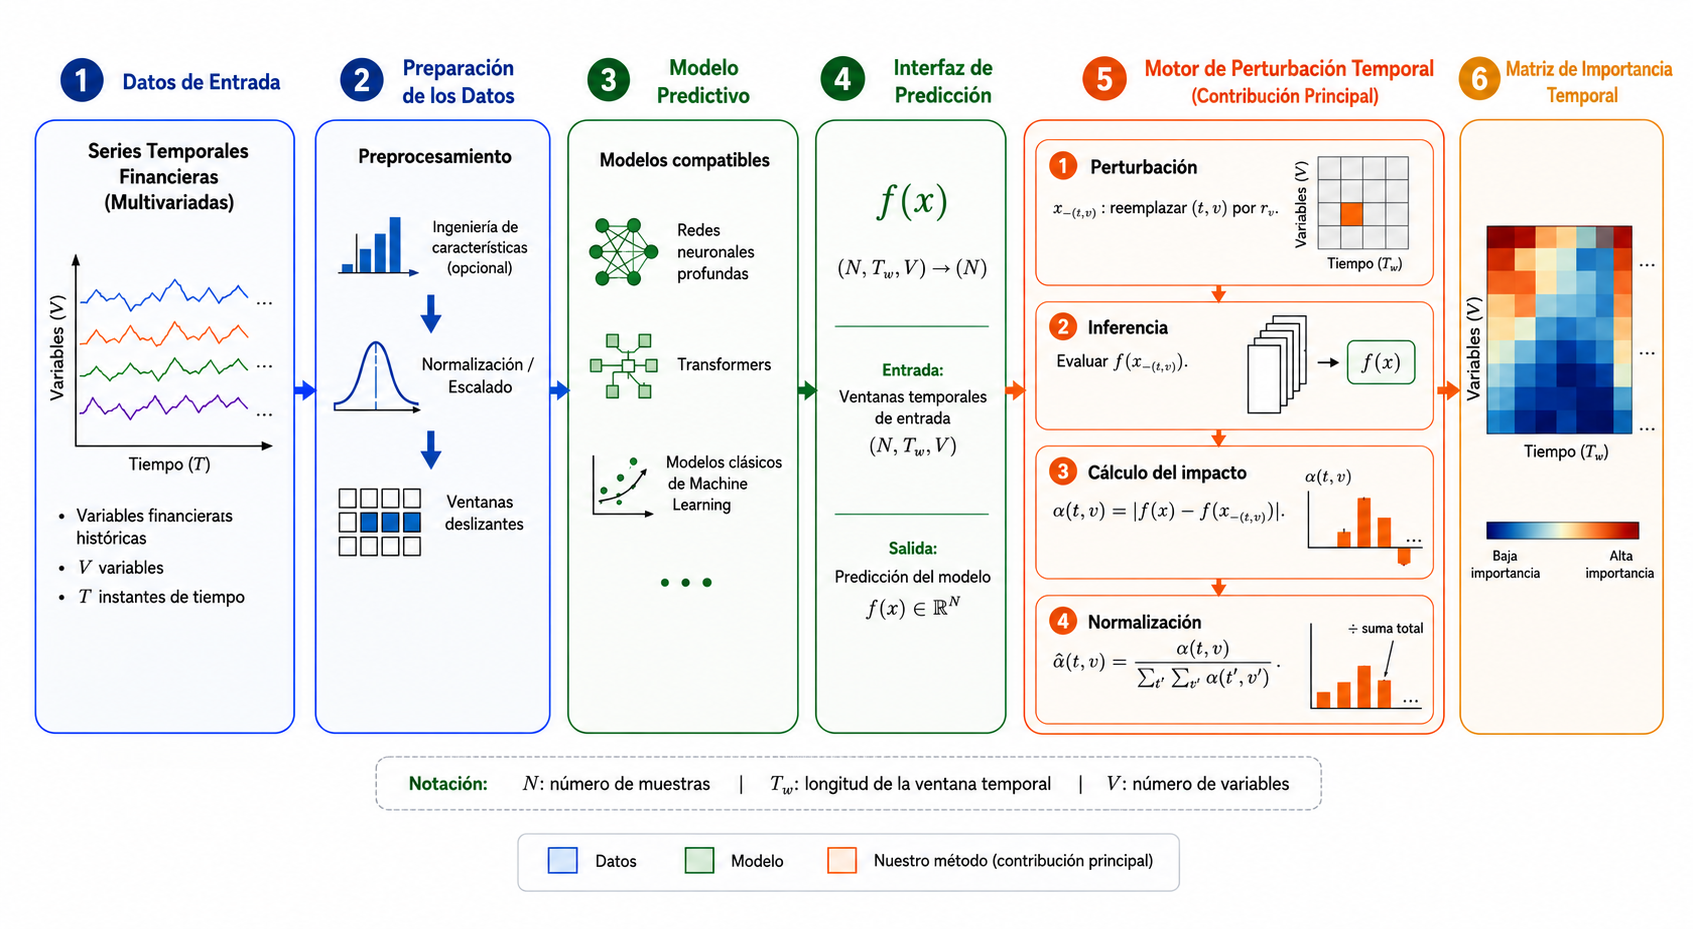
\includegraphics[width=\textwidth]{Graficos/PIPELINE.png}
\caption{Pipeline del framework en seis etapas. (1)~Datos de entrada, series temporales financieras multivariadas. (2)~Preparación de los datos, con ingeniería de características, normalización y ventanas deslizantes. (3)~Modelo predictivo, que puede ser una red neuronal, un Transformer o un modelo clásico de aprendizaje automático. (4)~Interfaz de predicción, que recibe ventanas de forma $(N,T,V)$ y devuelve $N$ predicciones. (5)~Motor de perturbación temporal, con perturbación de una celda, inferencia, cálculo del impacto y normalización. (6)~Matriz de importancia temporal $\hat{\alpha}$. En la figura, $T_w$ denota la longitud $T$ de la ventana.}
\label{fig:pipeline}
\end{figure}

\section{Objetivos Específicos}
\label{sec:objetivos_especificos}

\begin{enumerate}
    \item Diseñar una interfaz uniforme de predicción, mediante un patrón adaptador de dos niveles, que desacople el motor de perturbaciones de la estructura interna de cualquier modelo.
    \item Formular un motor de perturbaciones temporales que atribuya importancia a nivel de celda $(t,v)$, preservando el orden y la coherencia temporal del resto de la ventana, y cuyas perturbaciones sean independientes entre sí para poder evaluarse en un único batch paralelo en vez de una secuencia de pasos de optimización.
    \item Entrenar modelos de distinta naturaleza computacional (LSTM, Transformer, Random Forest) sobre el S\&P~500 como banco de pruebas del framework.
    \item Verificar que las explicaciones generadas reflejan el comportamiento específico de cada modelo, y no son independientes del modelo explicado ni artefacto del procedimiento, esperando mayor consistencia entre modelos de mecanismo similar (LSTM y Transformer) que frente a un modelo de mecanismo distinto (Random Forest). Esta expectativa de divergencia parcial, no de igualdad total, sigue el criterio de Adebayo et al.\ \cite{adebayo2018}, quienes muestran que un método de explicación que produce el mismo resultado sin importar el modelo explicado, incluso con sus pesos aleatorizados, no está reflejando ese modelo sino reproduciendo un artefacto propio del método. Que la atribución cambie con la arquitectura, en una proporción coherente con cuánto se parece su mecanismo interno al de otras arquitecturas evaluadas, es la evidencia a favor del framework, no una inconsistencia a corregir.
    \item Evaluar el framework frente al estado del arte agnóstico en precisión de identificación, consistencia entre modelos y velocidad de cómputo.
    \item Investigar si existe una consideración anclada en la estructura particular de Random Forest que reduzca su mayor sensibilidad observada al vector de referencia, y documentar el resultado con la misma rigurosidad tanto si confirma como si descarta la hipótesis.
\end{enumerate}

\section{Organización de la tesis}
\label{sec:organizacion_tesis}

El Capítulo~2 presenta el marco teórico, que parte de las series temporales financieras y los modelos que se entrenan sobre ellas, define la interpretabilidad y la explicabilidad, y formaliza la explicabilidad post-hoc, el agnosticismo al modelo, los métodos de perturbación, la explicabilidad temporal y los criterios de evaluación de una explicación. El Capítulo~3 revisa los trabajos relacionados de los últimos cinco años, organizados en tres ejes, los métodos de perturbación agnósticos que incorporan de algún modo la dimensión temporal, los frameworks explícitamente diseñados para ser temporalmente conscientes y agnósticos a la vez, incluyendo el linaje directo de DynaMask, y los explicadores aprendidos con objetivos de cuello de botella de información. El Capítulo~4 describe la propuesta, la interfaz uniforme de predicción, el motor de perturbaciones temporales, los tres modelos entrenados, y la investigación de una consideración específica para Random Forest. El Capítulo~5 presenta los resultados experimentales, desempeño predictivo, validación con ground truth sintético, verificación de agnosticismo sobre el S\&P~500, pruebas de robustez, y comparación con el estado del arte. El Capítulo~6 cierra con las conclusiones, las limitaciones del trabajo y el trabajo futuro planificado.
